\documentclass[12pt, a4papre]{article}
\usepackage[catalan]{babel}
\usepackage[unicode]{hyperref}
\usepackage{amsmath}
\usepackage{amssymb}
\usepackage{amsthm}
\usepackage{xifthen}
\usepackage{listings}
\usepackage{float}
\usepackage{siunitx}
\usepackage{graphicx}
\usepackage{indentfirst}

\newcommand{\norm}[1]{\lvert #1 \rvert}
\graphicspath{ {./Images/Memoria3/} }

\hypersetup{
    colorlinks = true,
    linkcolor = blue
}

\renewcommand{\figurename}{Fig.}

\author{Daniel Vilardell}
\title{Memoria Practica 3 FISE}
\date{}

\begin{document}
	\maketitle
	
	\textbf{Qüestió 1.1:} Es pot veure a la imatge que la frequencia central del filtre es de $1kHz$, cosa que cuadra amb el que es va comentar al estudi previ, ja que tenim que $w_o = \frac{1}{RC}$.

	\begin{figure}[H]
		\begin{center}
		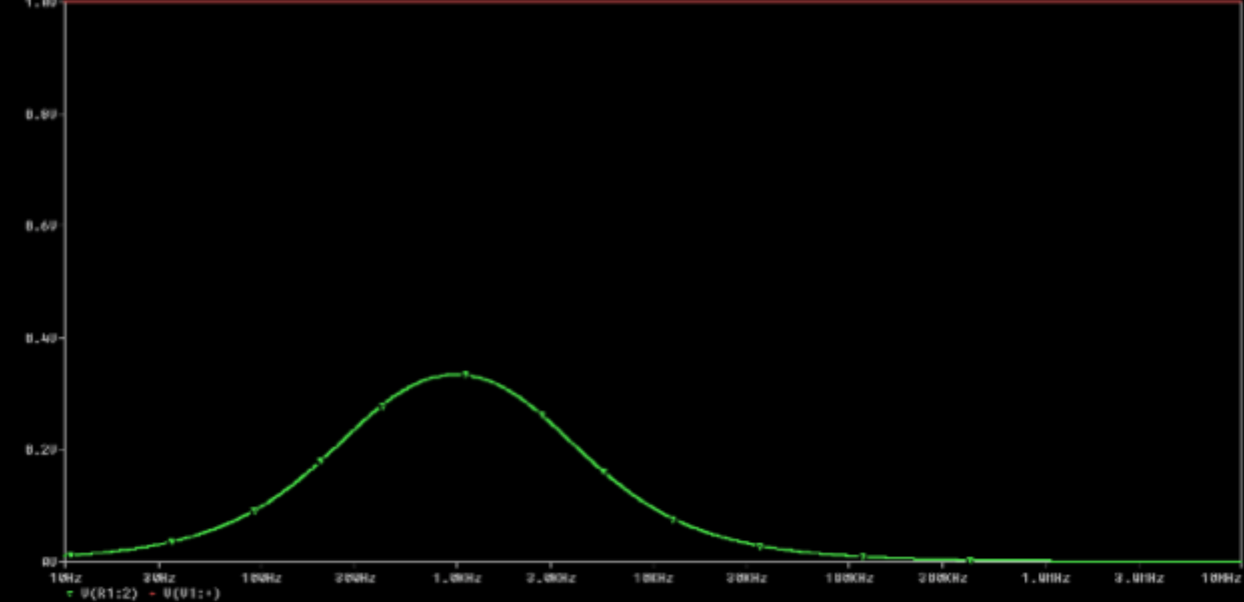
\includegraphics[width=110mm]{1_1.PNG}
		\end{center}
	\end{figure}
	
	\textbf{Qüestió 2.1:} Trivialment es pot veure en les seguents captures que amb el filtre passiu obtenim les mateixes respostes que al apartat anterior, es cuan realimentem el filtre que obtenim un guany bastant superior, mantenint pero el ample de banda, així fent un filtre mes selectiu i amb un factor de qualitat mes elevat.
	
	Els pols complexes fan que el filtre sigui mes selectiu i tingui un ample de banda inferior, i així obtenint un factor de qualitat millor.
	
	\begin{figure}[H]
		\begin{center}
		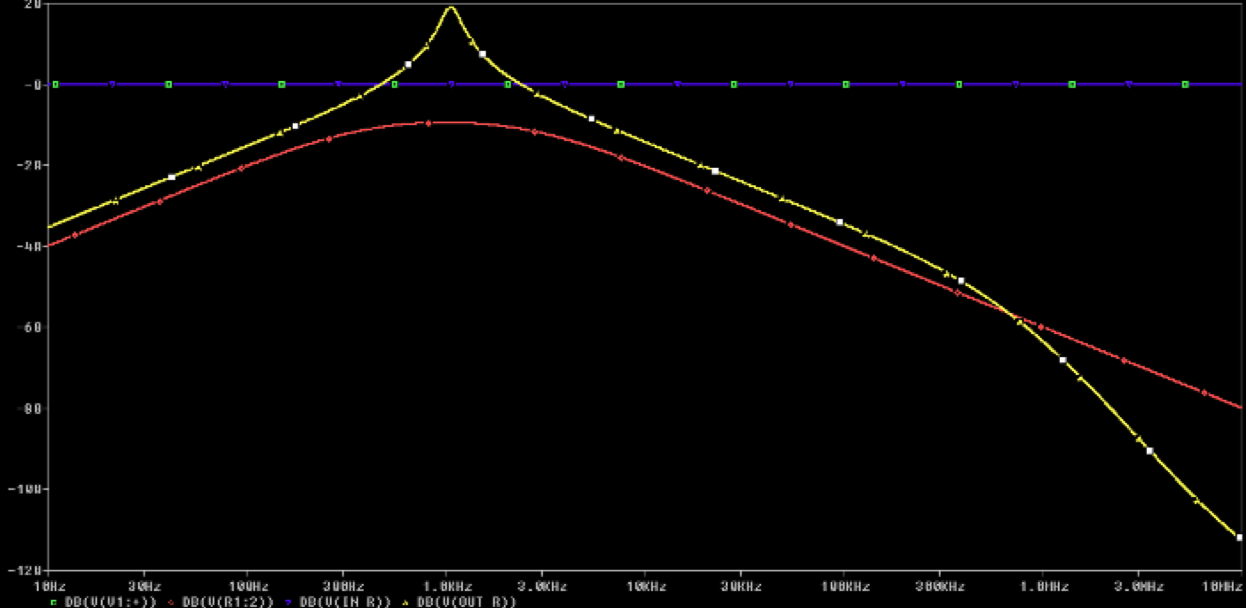
\includegraphics[width=110mm]{2_1.png}
		\end{center}
	\end{figure}
	
	\begin{figure}[H]
		\begin{center}
		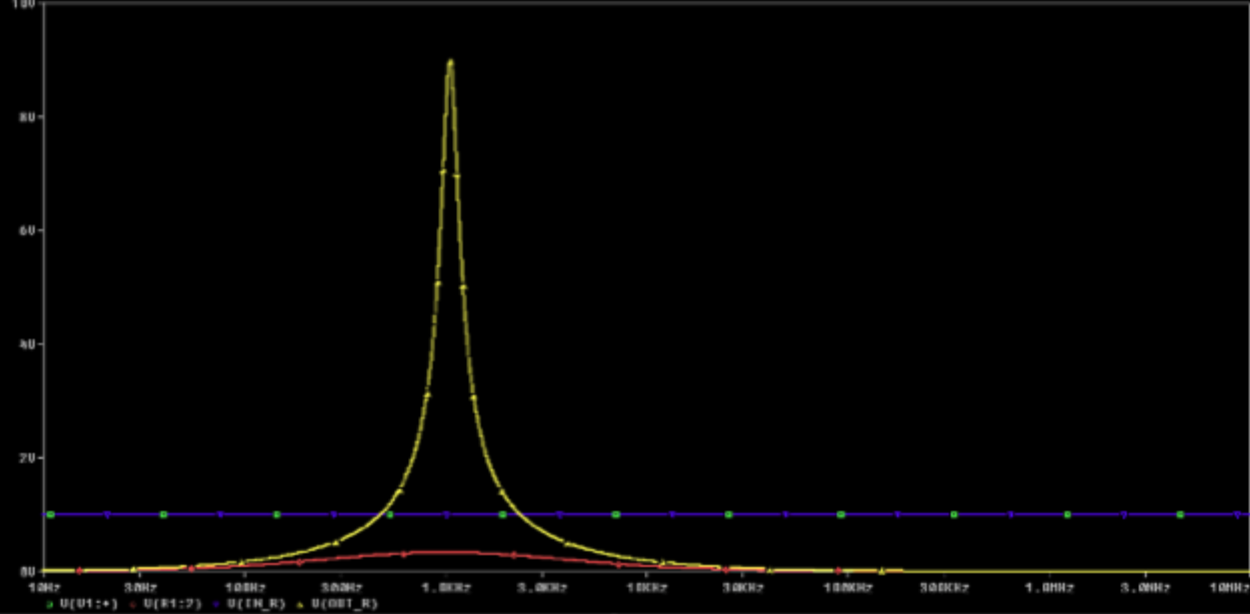
\includegraphics[width=110mm]{2_1_2.png}
		\end{center}
	\end{figure}
	\begin{figure}[H]
		\begin{center}
		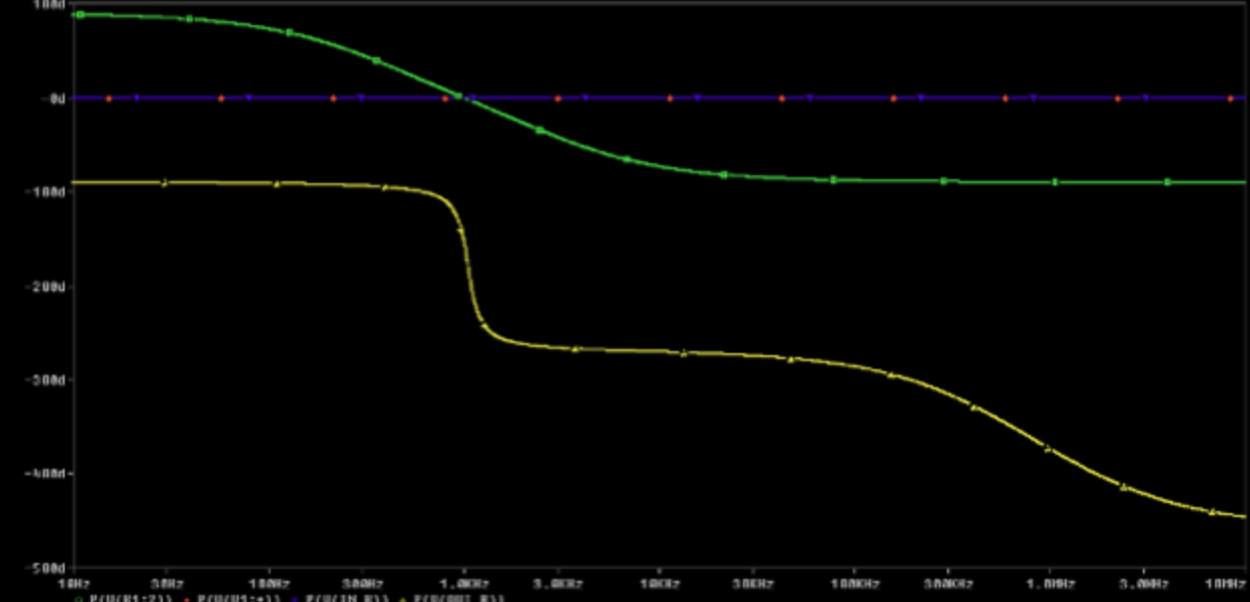
\includegraphics[width=110mm]{2_1_3.png}
		\end{center}
	\end{figure}
	
	\textbf{Qüestió 2.2:} Tal i com es veu a les següents imatges si que es pot fer, i d'aquesta forma obtindriem un filtre amb un guany menor centrat a 100kHz pero mantenint l'ample de banda i el factor de qualitat.
	
	\begin{figure}[H]
		\begin{center}
		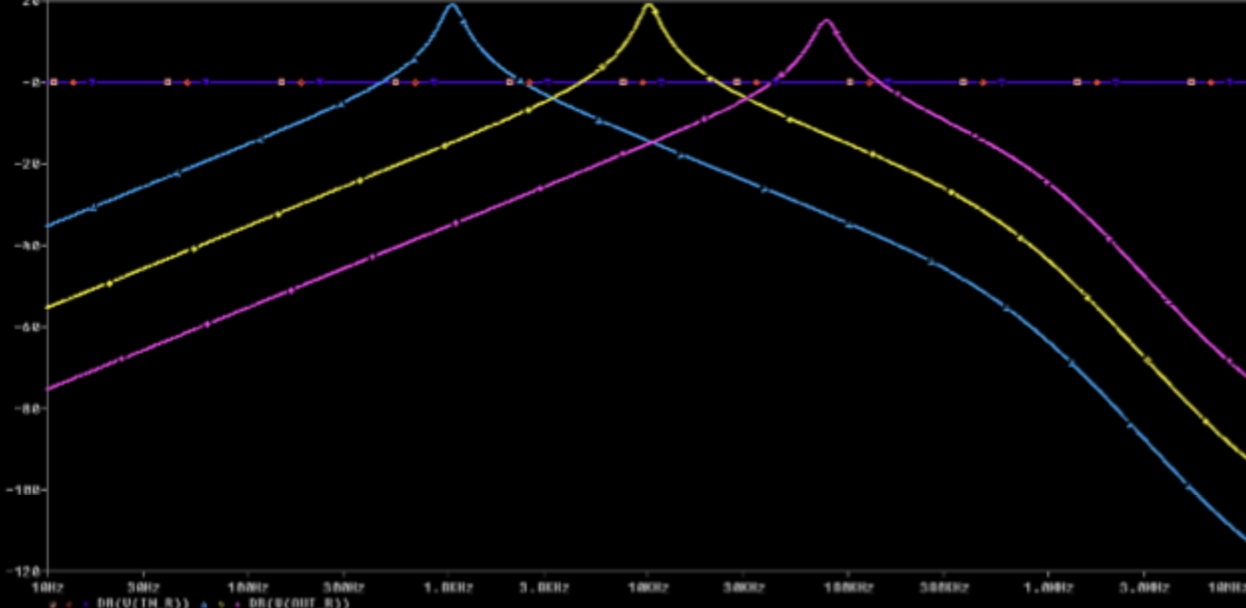
\includegraphics[width=110mm]{2_2_1.png}
		\end{center}
	\end{figure}
	
	\begin{figure}[H]
		\begin{center}
		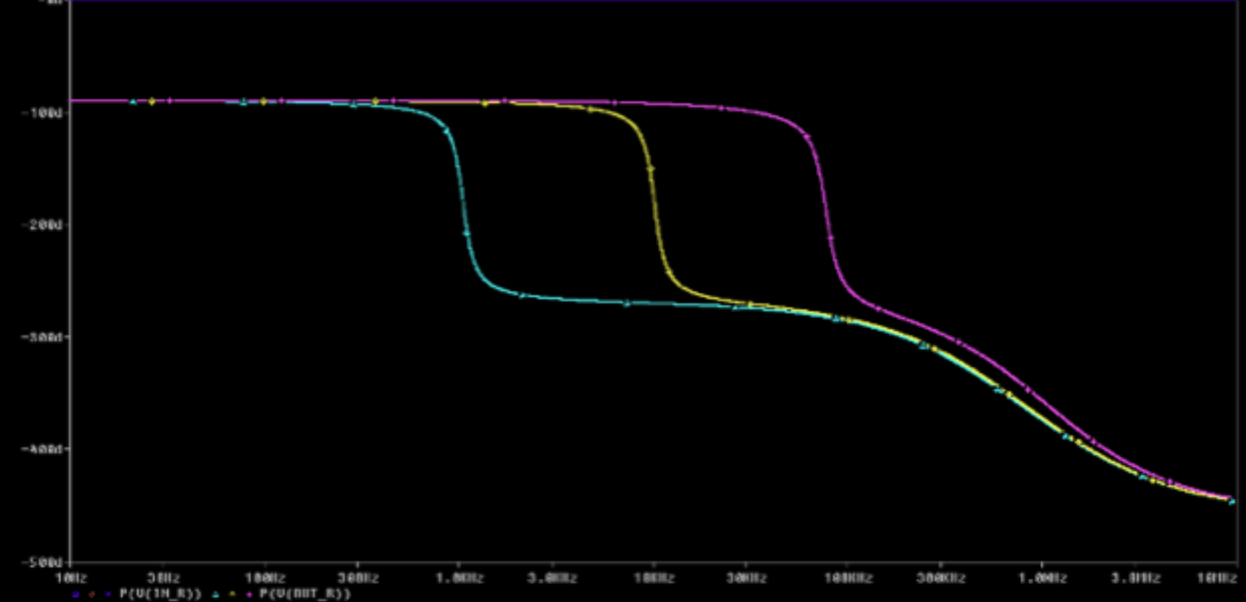
\includegraphics[width=110mm]{2_2_2.png}
		\end{center}
	\end{figure}
	
	\textbf{Qüestió 2.3:} Podem veure que amb un factor de qualitat $Q = 5$ obtenim un guany de 19dB i amb un $Q = 10$ obtenim un guany de 25dB. Tot i que la frequencia central es mante les fases presenten una petita diferencia.
	
	\begin{figure}[H]
		\begin{center}
		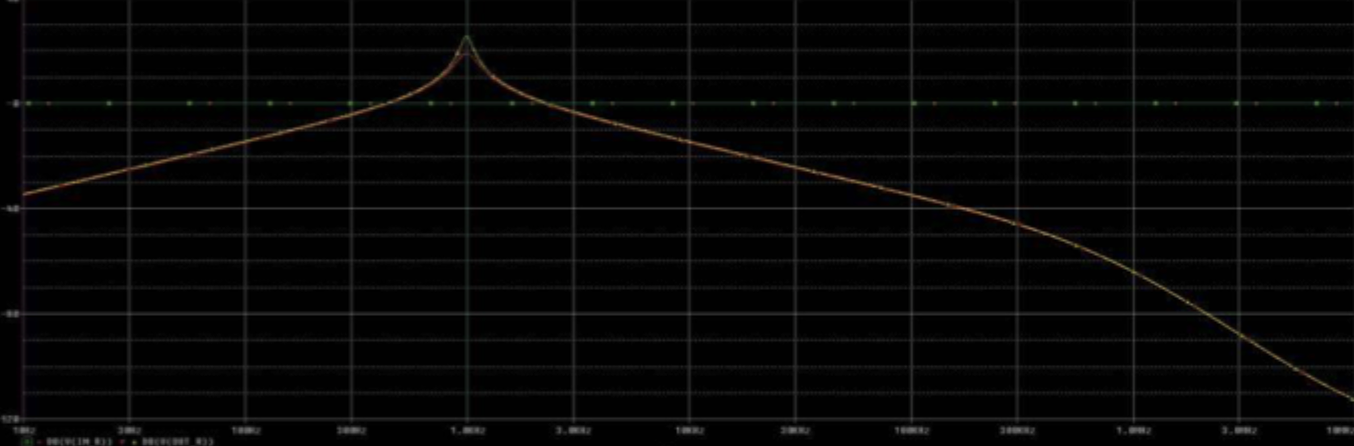
\includegraphics[width=110mm]{2_3_1.png}
		\end{center}
	\end{figure}
	
	\begin{figure}[H]
		\begin{center}
		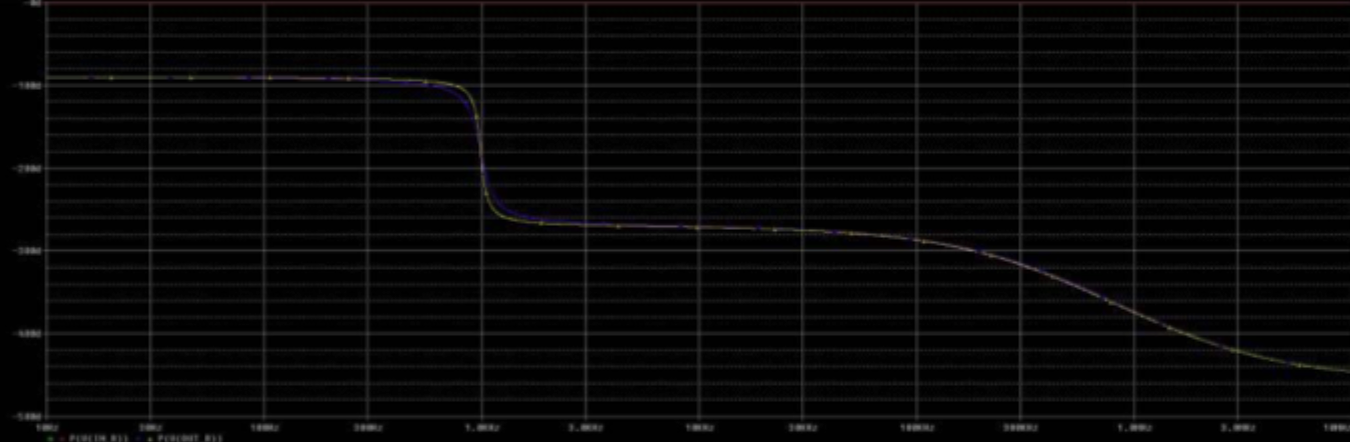
\includegraphics[width=110mm]{2_3_2.png}
		\end{center}
	\end{figure}
	
	\textbf{Qüestió 3.1:} El temps transitori es veu a la grafica que es de aproximadament $6ms$. A la grafica de la FFT podem veure que la relació entre el primer i el tercer harmonic amb el filtre realimentat es de 40, molt millor que el que obtenim de 10 amb el filtre no realimentat. Això es deu a que aquest primer te un factor de qualitat mes elevat tal i com hem comentat a la questió 2.
	
	\begin{figure}[H]
		\begin{center}
		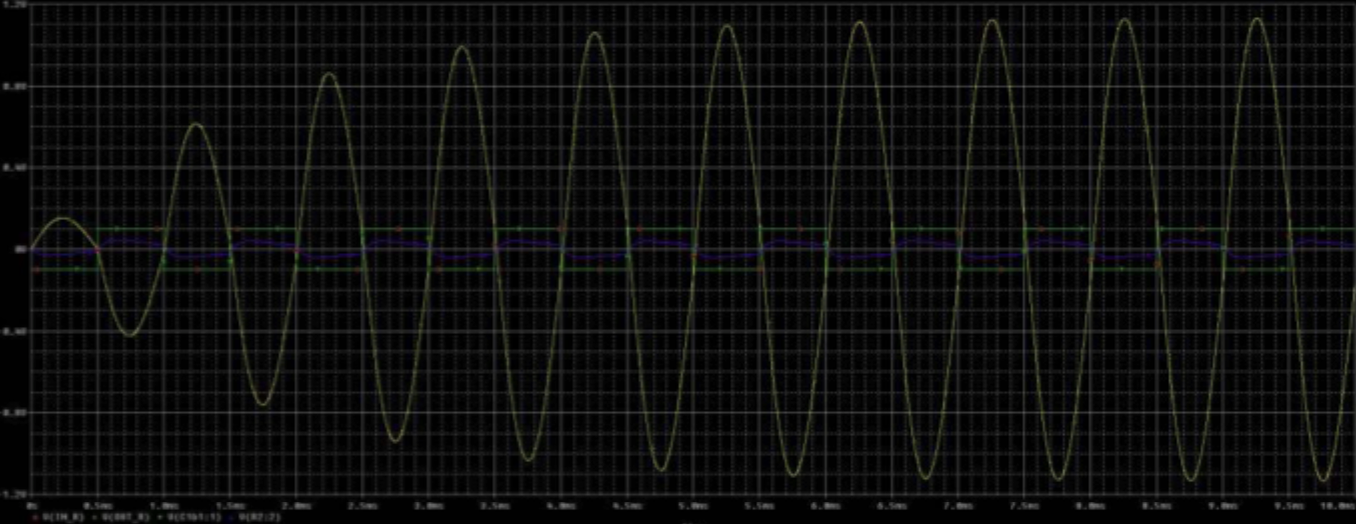
\includegraphics[width=110mm]{3_1_1.png}
		\end{center}
	\end{figure}
	
	\begin{figure}[H]
		\begin{center}
		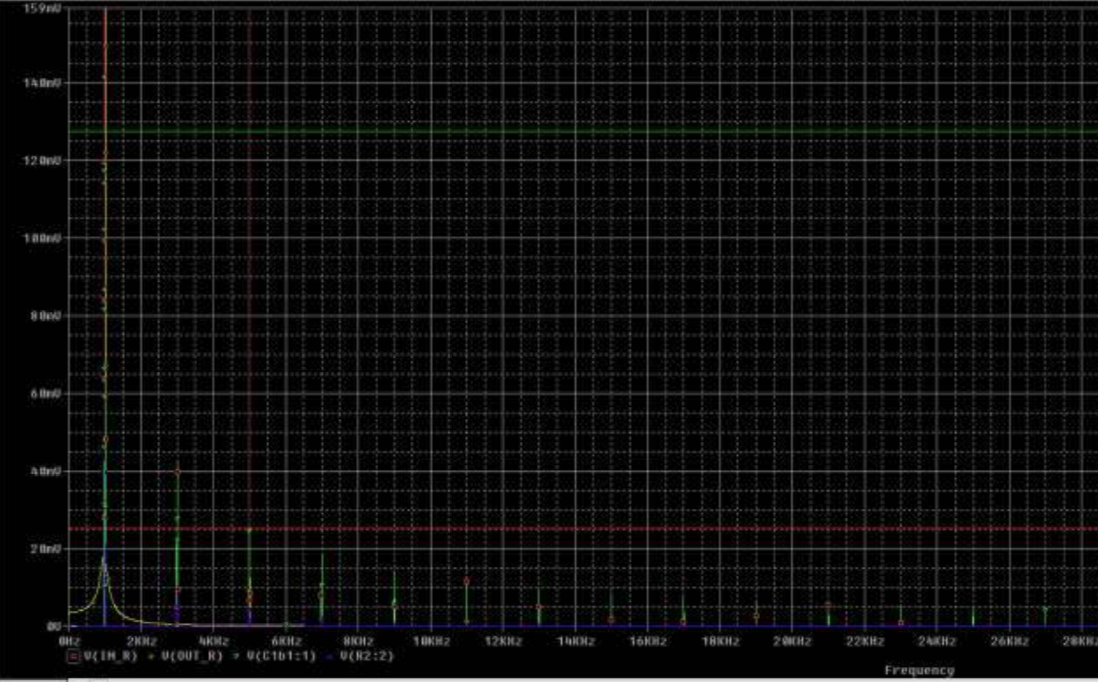
\includegraphics[width=110mm]{3_1_2.png}
		\end{center}
	\end{figure}
	
	\textbf{Qüestió 3.2:} Ara la durada del transitori es de 10ms, mes elevada que amb el de $Q = 5$, i el filtre te una selectivitat mes elevada.
	
	\begin{figure}[H]
		\begin{center}
		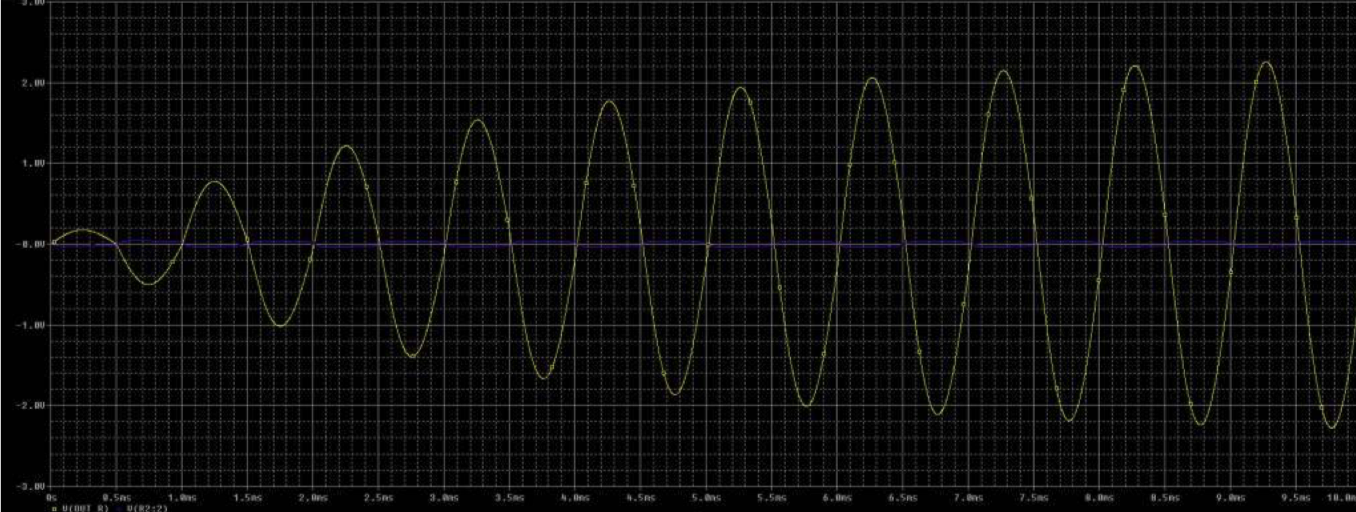
\includegraphics[width=110mm]{3_2_1.png}
		\end{center}
	\end{figure}
	
	\textbf{Qüestió 4.1:} L'amplitud teorica que s'hauria d'esperar a la simulació es de 9V, tot i que la obtinguda es de 5.5V. Es pot veure que degut als errors del amplificador com pot ser el SR presenta forta distorció respecte al senyal d'entrada.
	
	\begin{figure}[H]
		\begin{center}
		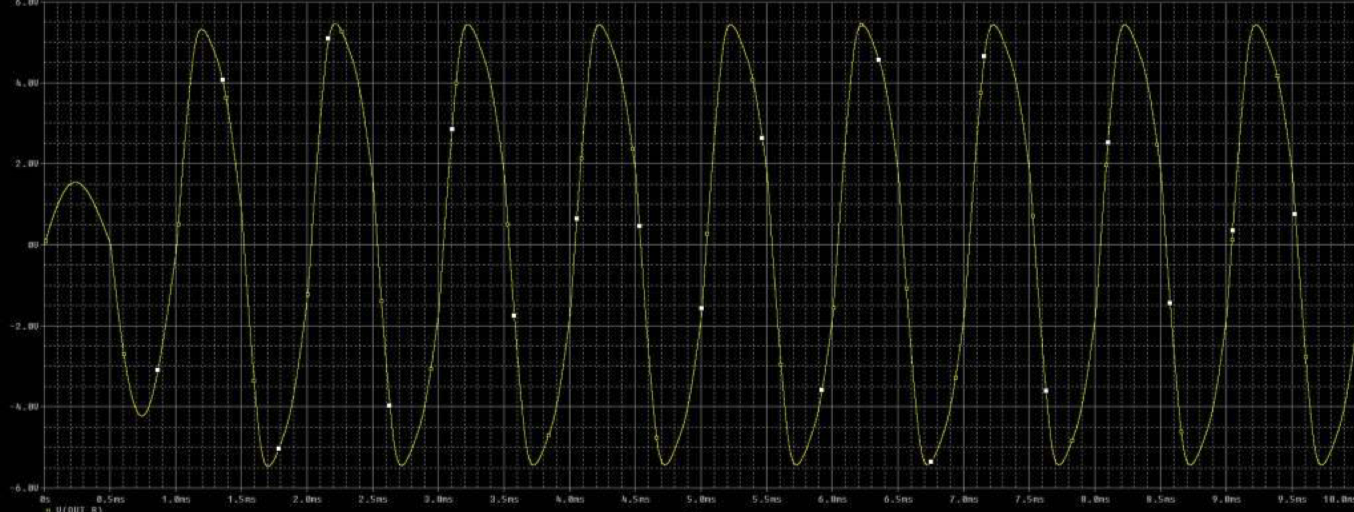
\includegraphics[width=110mm]{4_1.png}
		\end{center}
	\end{figure}
	
	\textbf{Qüestió 4.2:} Es pot veure rapidament que el senyal de sortida superaria la tensió de saturació, per tant la distorció principal es provocada per aquest fet, ja que podem observar que les parts superiors i inferiors de les sinusoides son planes.
	
	\begin{figure}[H]
		\begin{center}
		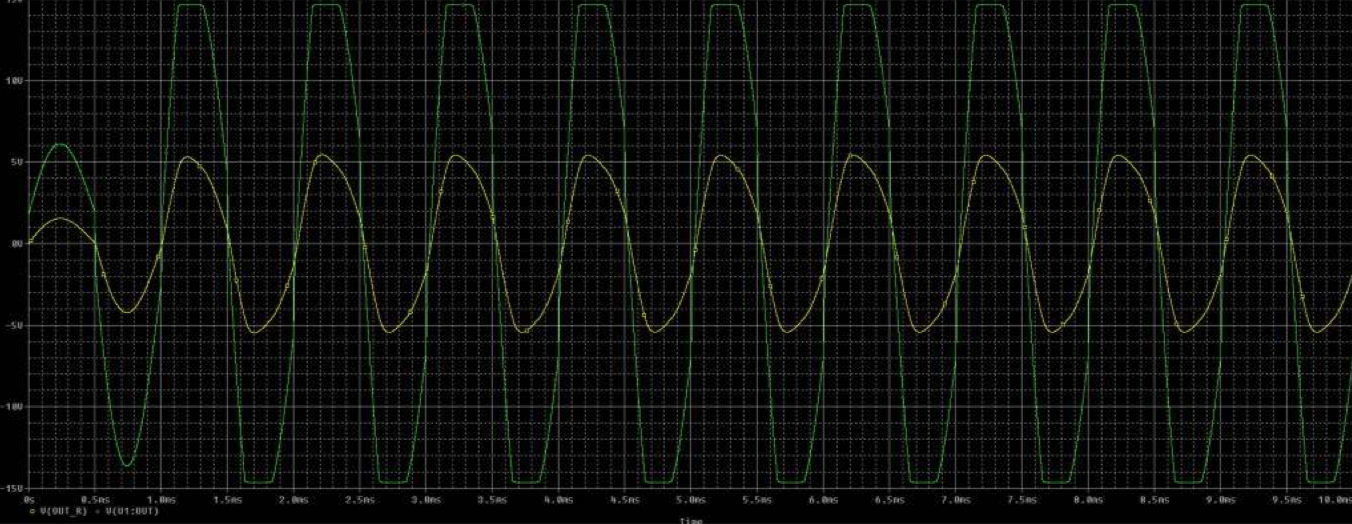
\includegraphics[width=110mm]{4_2.png}
		\end{center}
	\end{figure}
	
	\textbf{Qüestió 5.1:} Podem veure que el circuit ara es inestable, i degut a aixo el diagrama de fase es veu alterat, ja que els pols ara estan al semipla positiu de w real. Quan el guany es maxim, la fase passa de -90º a 90º.
	
	\begin{figure}[H]
		\begin{center}
		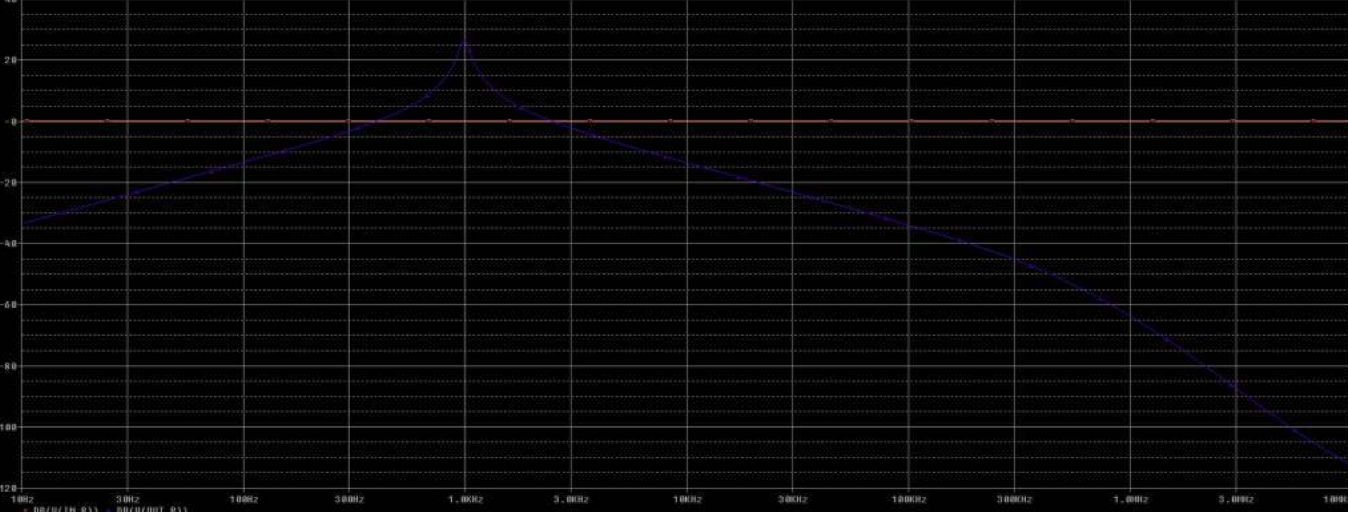
\includegraphics[width=110mm]{5_1.png}
		\end{center}
	\end{figure}
	
	\begin{figure}[H]
		\begin{center}
		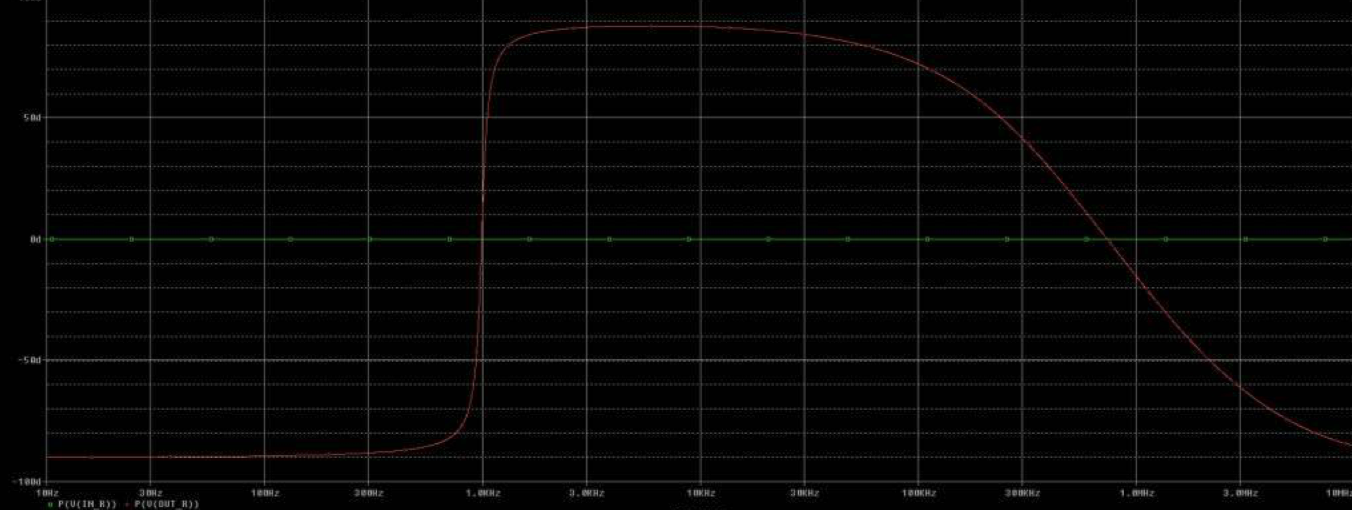
\includegraphics[width=110mm]{5_1_2.png}
		\end{center}
	\end{figure}
	
	\textbf{Qüestió 5.2:} Ara observem que tot i el senyal a la sortida del amplificador estar saturat, el de sortida del circuit no ho esta, i oscila amb una amplitud de aproximadament $5V$.
	
	\begin{figure}[H]
		\begin{center}
		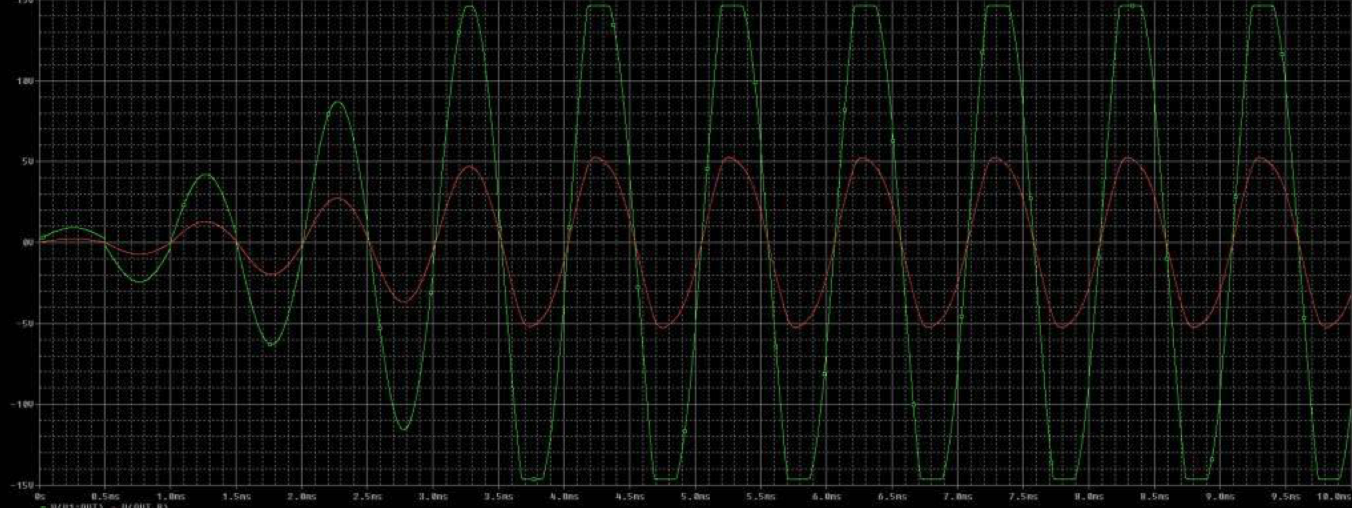
\includegraphics[width=110mm]{5_2.png}
		\end{center}
	\end{figure}
	
	\textbf{Qüestió 5.3:} Al tenir el senyal quadrat de mes frecuencia, provoca una petita distorció a la sortida del circuit i augmenta el estat transitori d'aquest.
	
	\begin{figure}[H]
		\begin{center}
		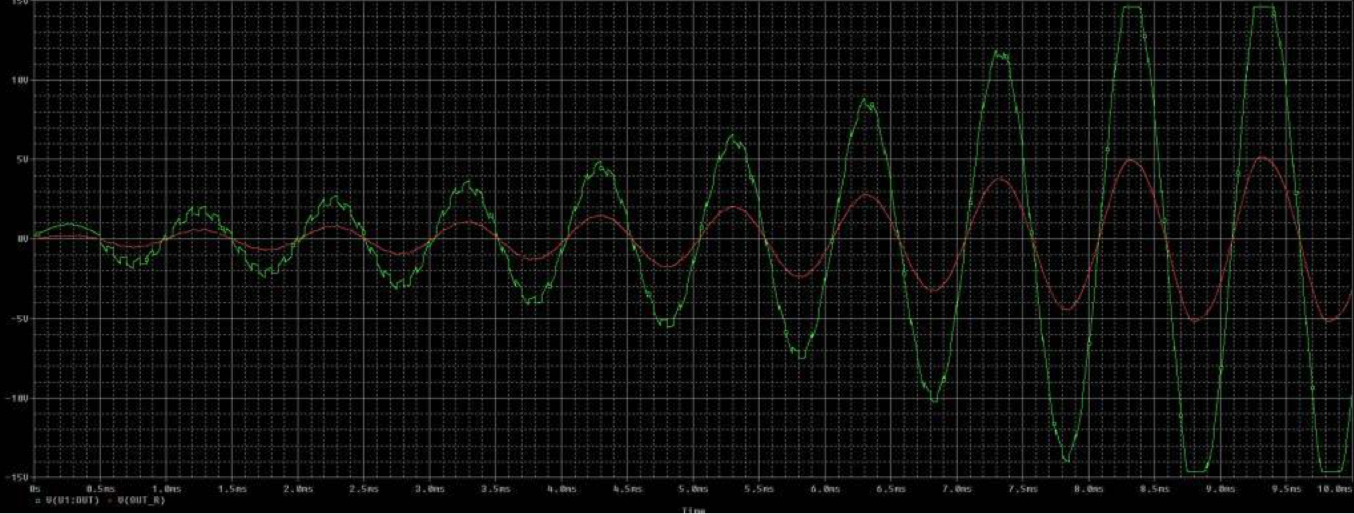
\includegraphics[width=110mm]{5_3_1.png}
		\end{center}
	\end{figure}
	
	\begin{figure}[H]
		\begin{center}
		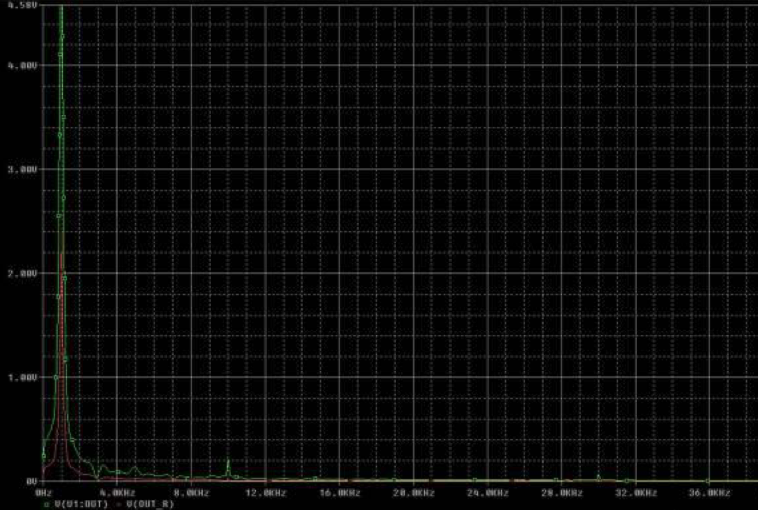
\includegraphics[width=110mm]{5_3_2.png}
		\end{center}
	\end{figure}
	
	\textbf{Qüestió 5.4:} Ara veiem a partir de la simulació i despres del periode transitori que la frequencia en la que esta oscilant el circuit es a 1025kHz. Un cop arriba al regim permanent es mante oscilant, just quan el AO entra en saturació.
	
	\begin{figure}[H]
		\begin{center}
		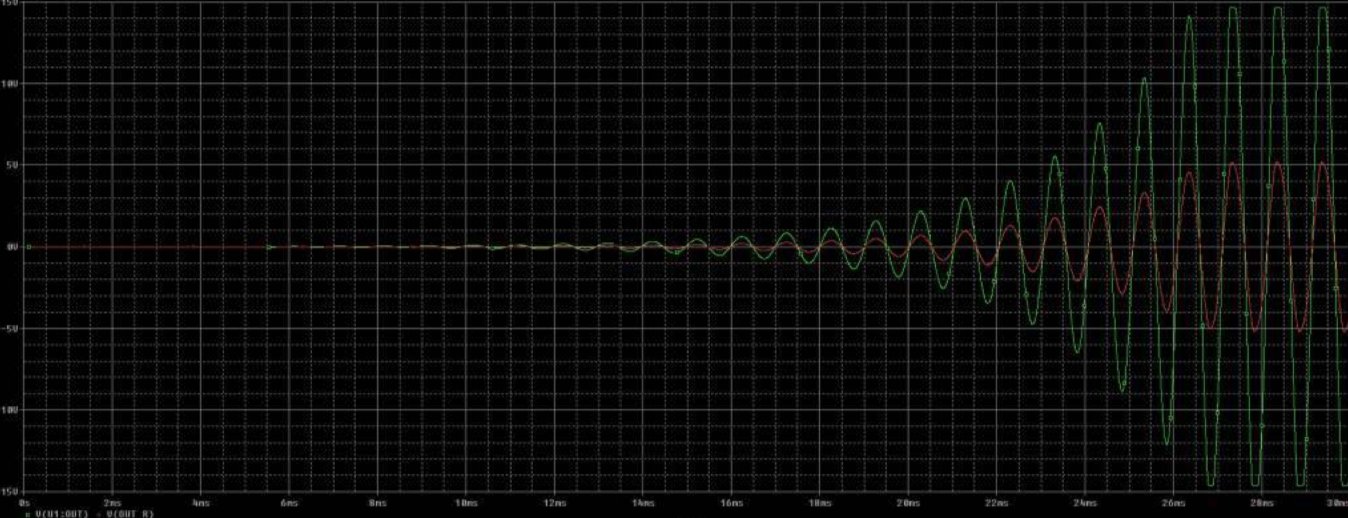
\includegraphics[width=110mm]{5_4.png}
		\end{center}
	\end{figure}
	
	\textbf{Qüestió 6.1:} En el cas que els 2 diodes estiguin en tall tindrem un guany $G = 1 + \frac{22k}{10k}$. Si un dels dos condueix tindrem un guany de $G = 1 + \frac{22k||R_{Adjust}}{10k}$.
	
	\textbf{Qüestió 6.2:} 
	
	\begin{itemize}
		\item Si $R = 50k$ el quocient val 3 quan $V_{in} = 197mV$.
		\item Si $R = 75k$ el quocient val 3 quan $V_{in} = 240mV$.
		\item Si $R = 100k$ el quocient val 3 quan $V_{in} = 300mV$.
	\end{itemize}
	
	\begin{figure}[H]
		\begin{center}
		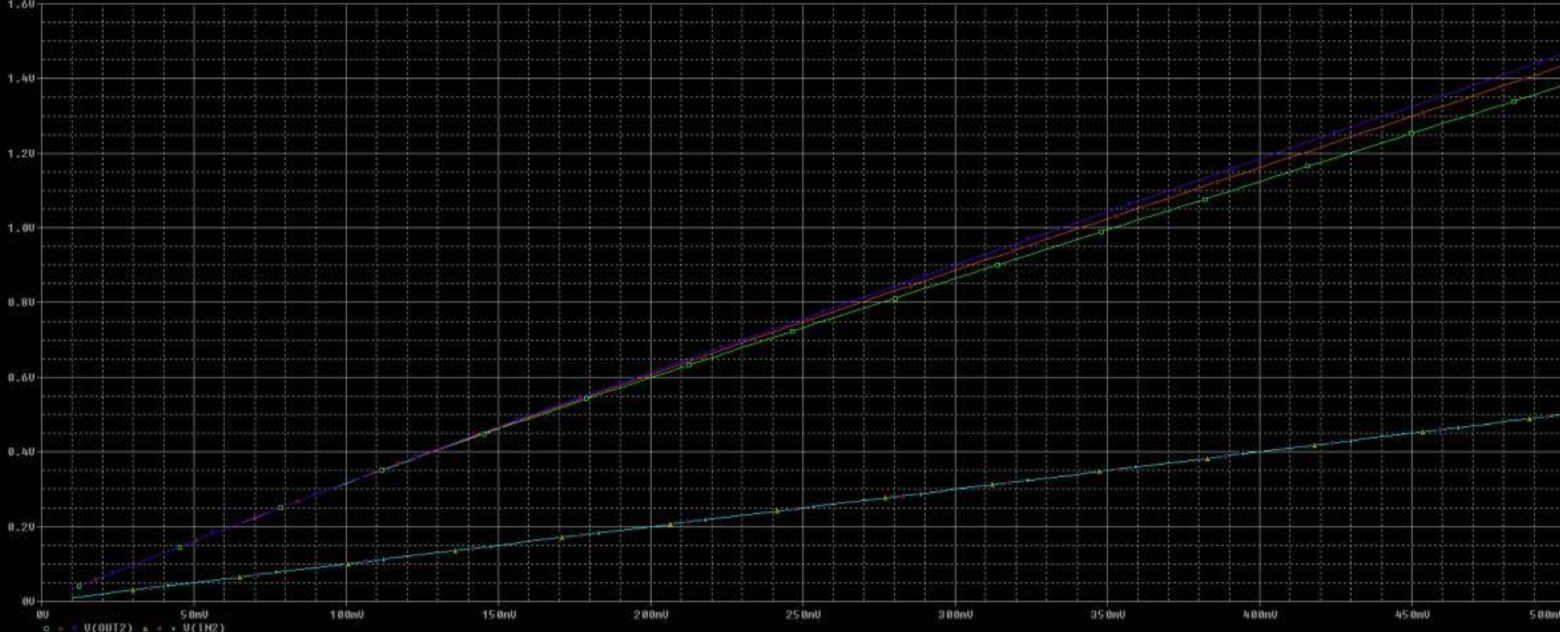
\includegraphics[width=110mm]{6_2.png}
		\end{center}
	\end{figure}
	
	\textbf{Qüestió 7.1:} 
	
	\begin{itemize}
		\item Si $R = 50k$ l'amplitud es de 1V.
		\item Si $R = 75k$ l'amplitud es de 0.7V.
		\item Si $R = 100k$ l'amplitud es de 0V.
	\end{itemize}
	
	\begin{figure}[H]
		\begin{center}
		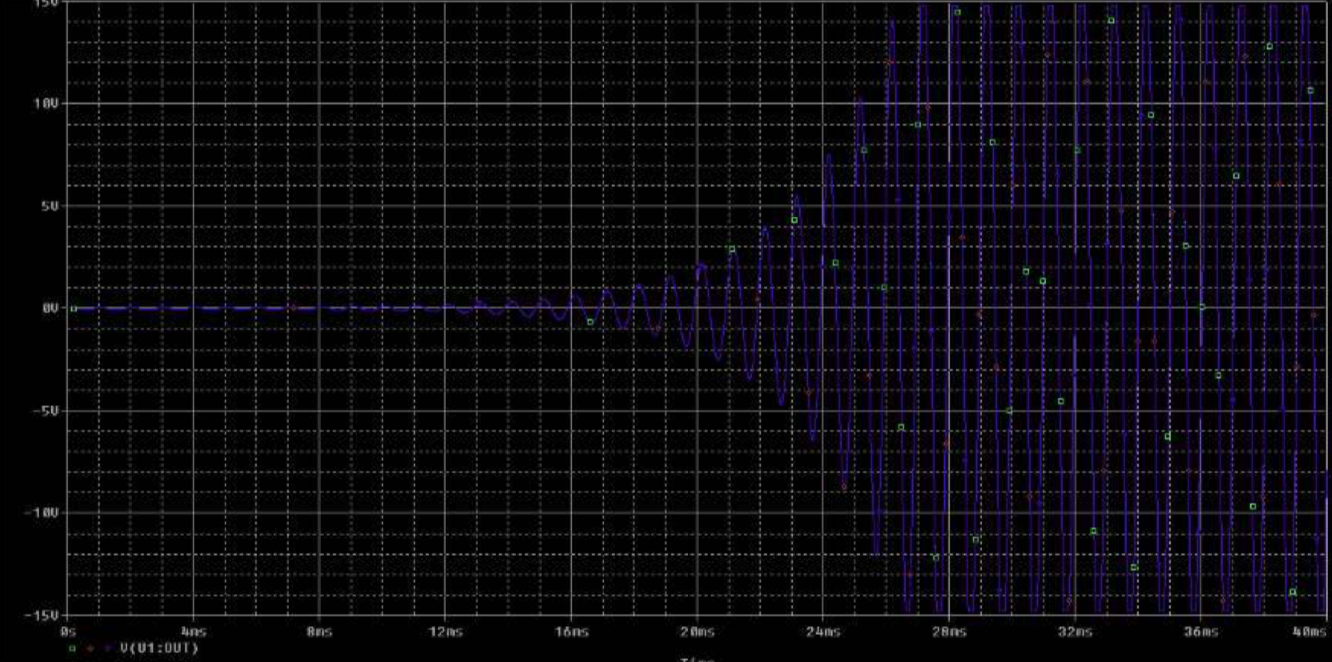
\includegraphics[width=110mm]{7_1.png}
		\end{center}
	\end{figure}
	
	\textbf{Qüestió 8.1:} $F_c = \frac{1}{2\pi RC} = 723.43Hz$
	
	\textbf{Qüestió 8.2:} Canviant els valors de la resistencia variable hem obtingut que oscil·la al voltant de $9.5k\si{\ohm}$.
	
	Per acabar la practica adjunto les imatges a on es mostra la sortida del circuit sense el pont de diodes, on es pot veure que la sortida esta distorssionada ja que el amplificador se satura, en canvi un cop afegim el pont de diodes evitem que arribi a la saturació i es veu com oscila adecuadament.
	
	\begin{figure}[H]
		\begin{center}
		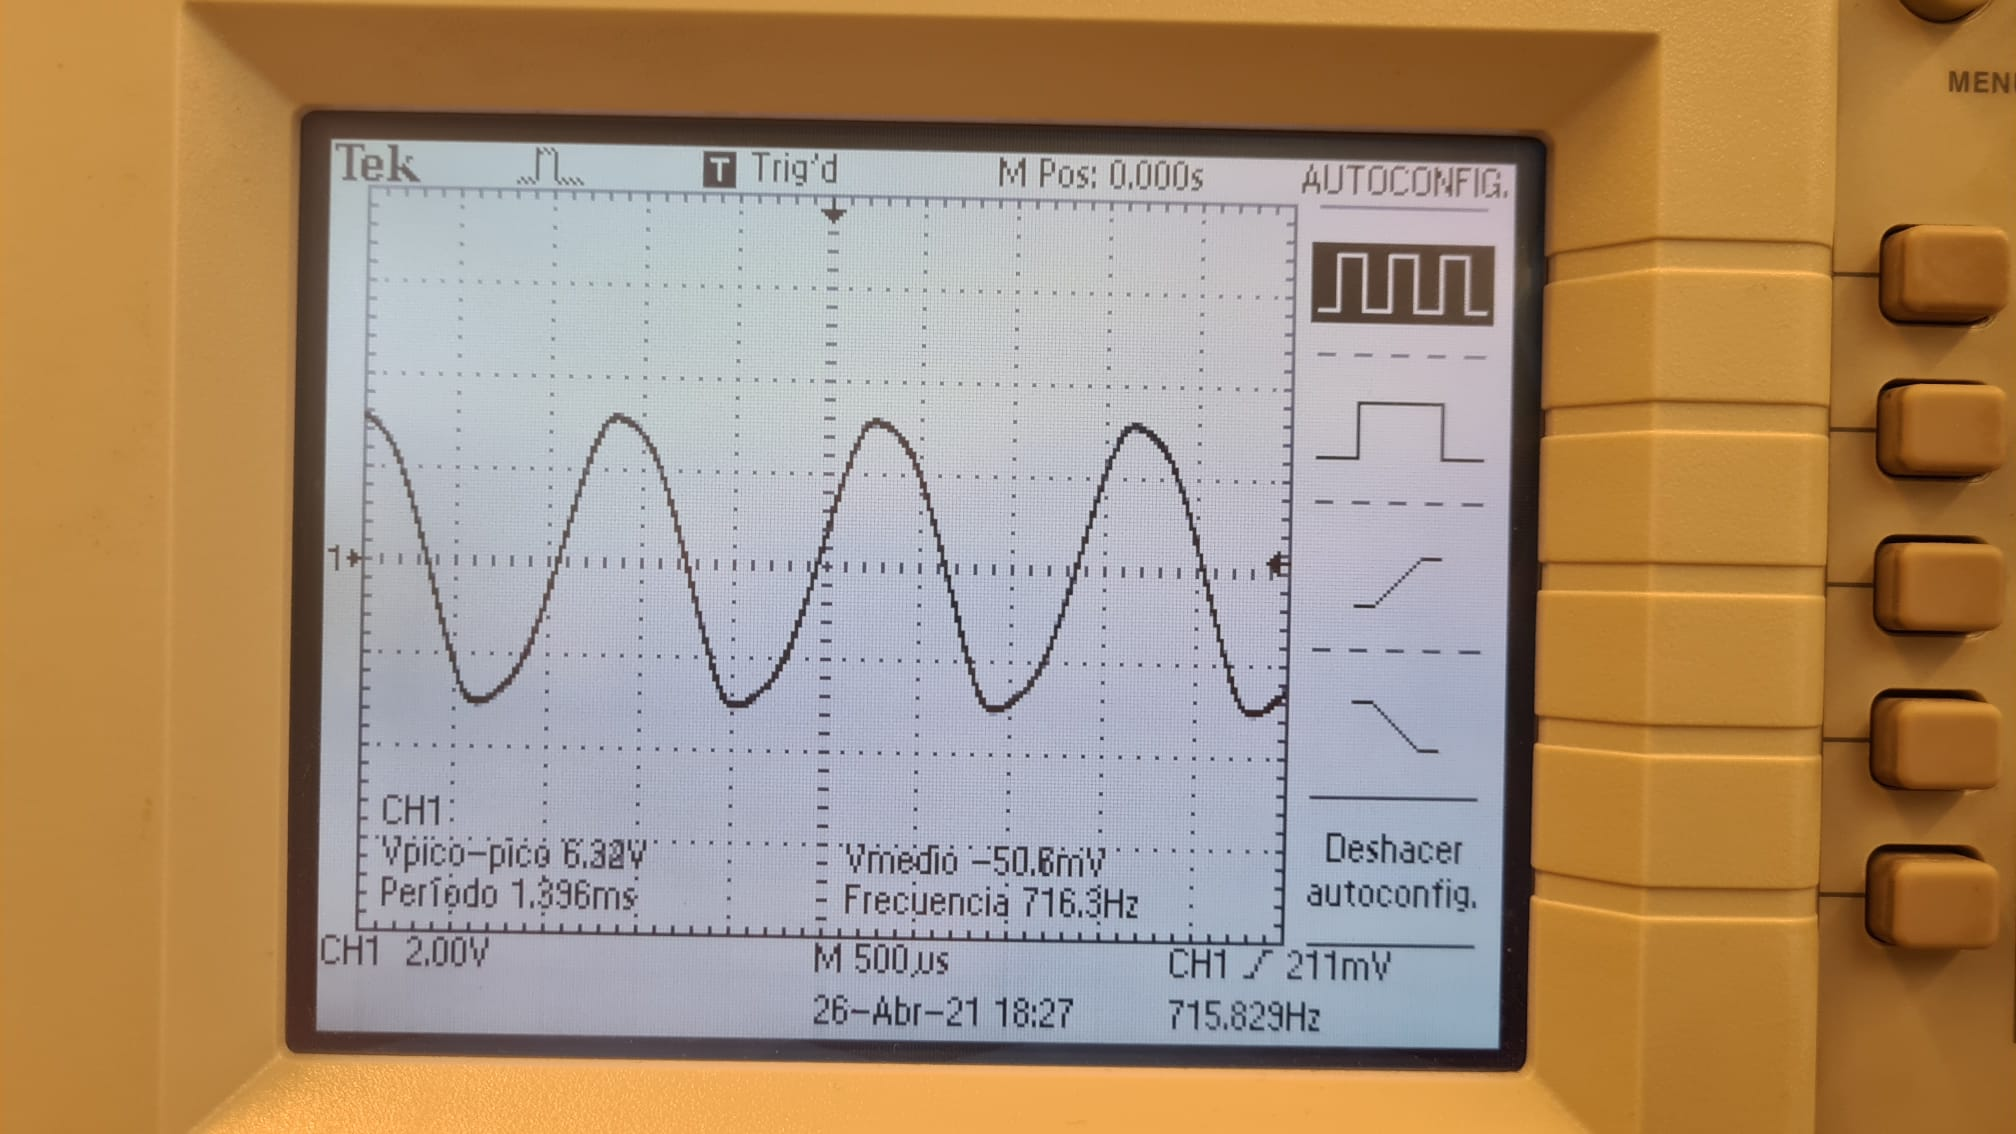
\includegraphics[width=110mm]{8_1.jpeg}
		\end{center}
	\end{figure}
	
	\begin{figure}[H]
		\begin{center}
		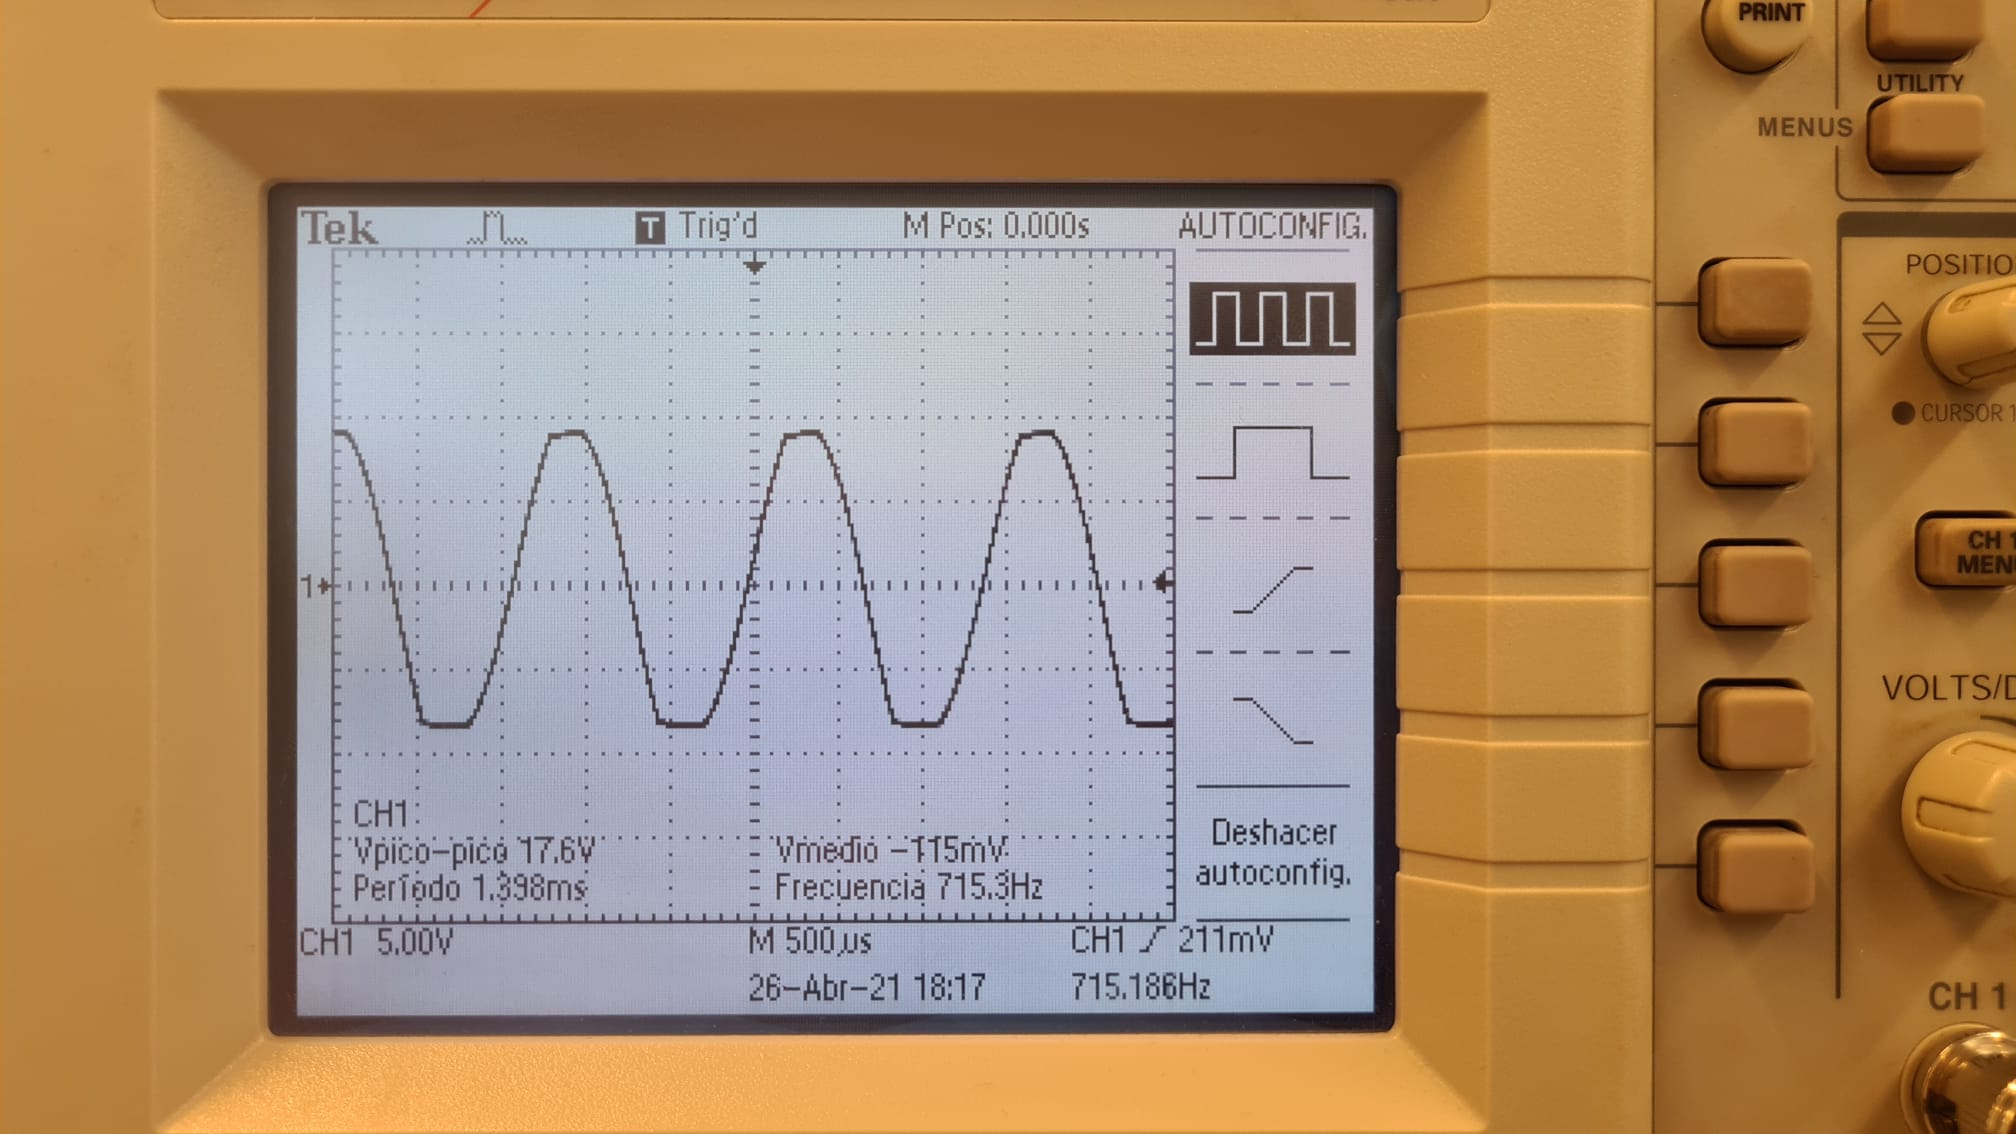
\includegraphics[width=110mm]{8_2.jpeg}
		\end{center}
	\end{figure}
	
	Veiem també a la seguent imatge la forma que te el circuit abans d'afegir el pont de diodes a la placa.
	
	\begin{figure}[H]
		\begin{center}
		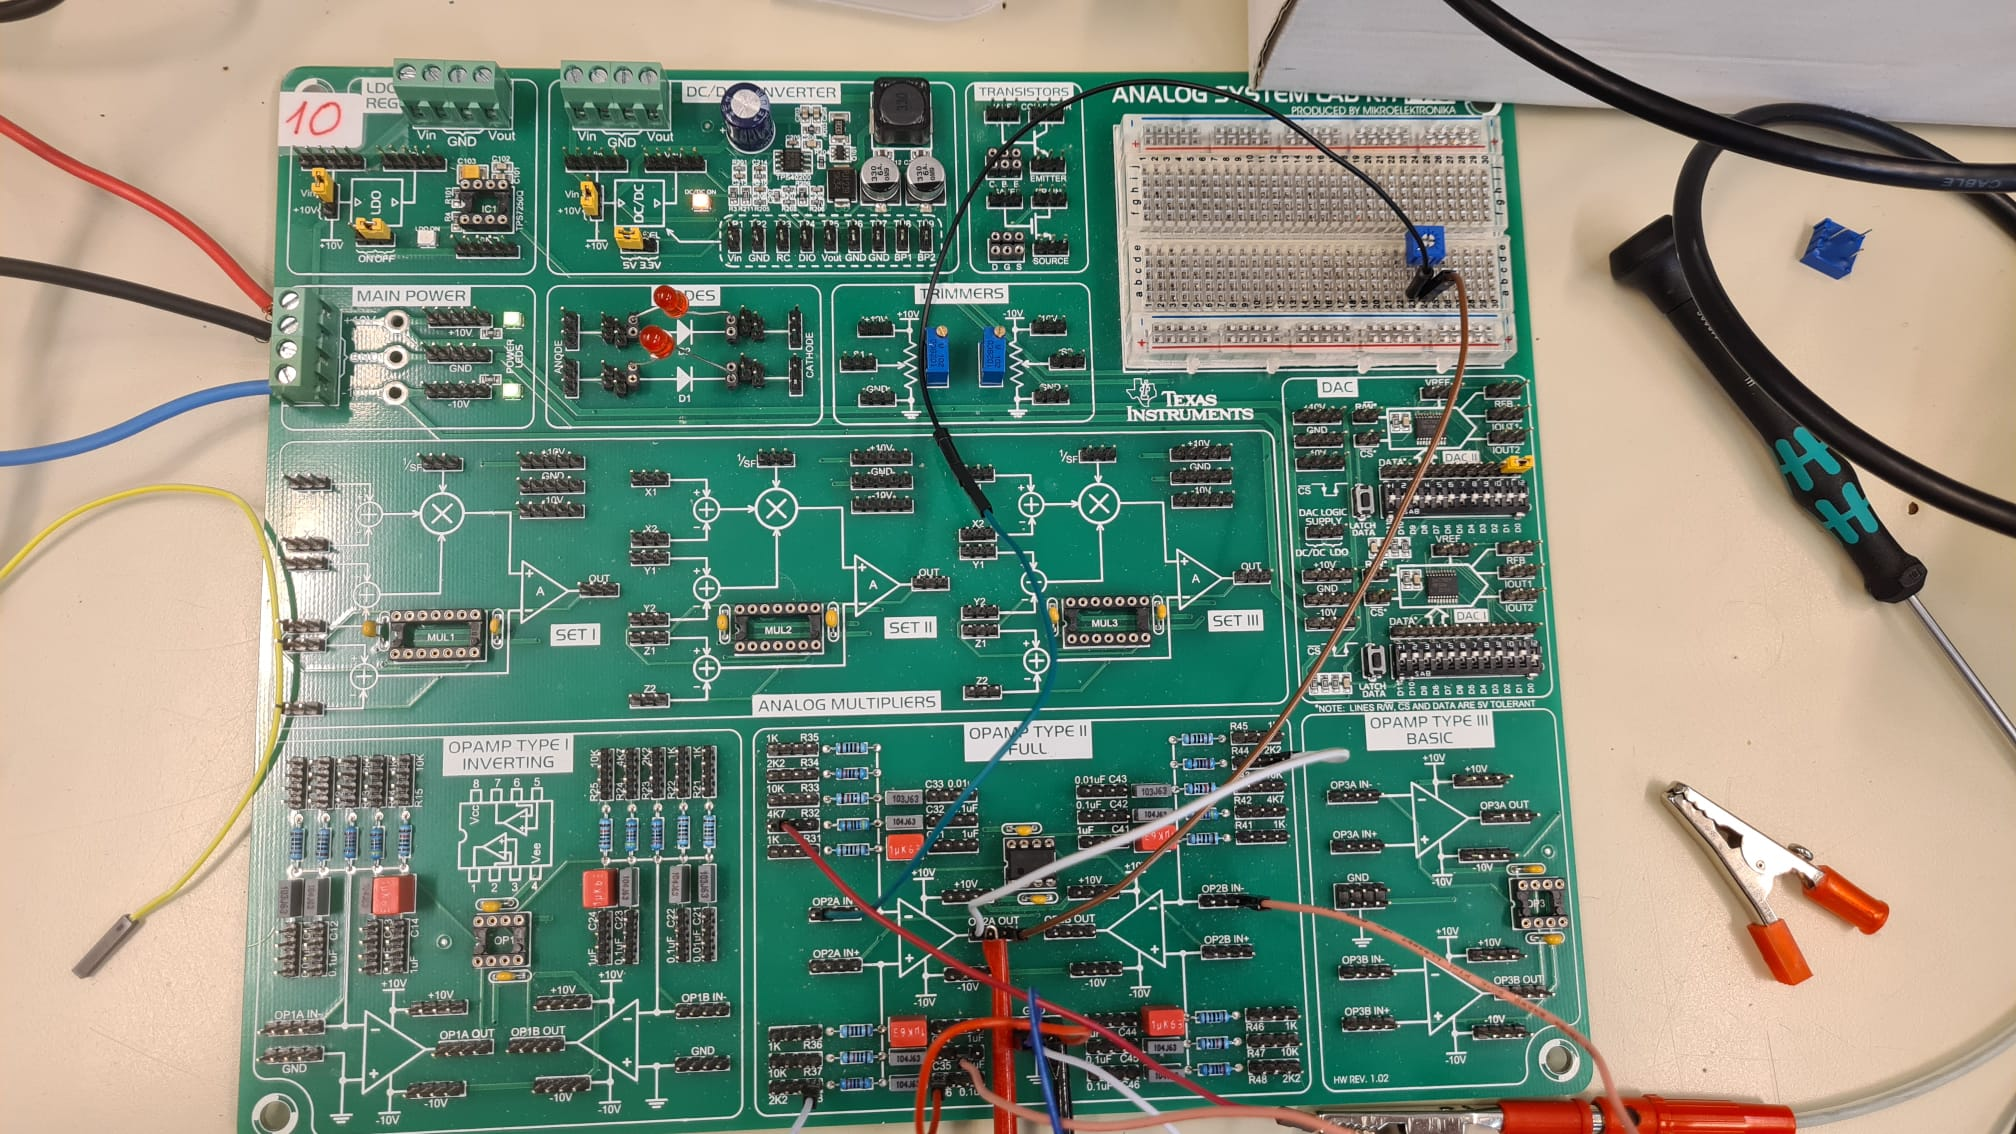
\includegraphics[width=110mm]{8_3.jpeg}
		\end{center}
	\end{figure}
	
\end{document}










